\documentclass[letterpaper]{article}
\usepackage{settings}

\begin{document}
\begin{notes}{Part 4: Geometry and Camera Models}

\NoteChapter{Image Warping and Stitching}

\NoteSection{Image Warping}

Applying a geometric transformation to an image requires deciding how to compute pixel values at non-integer locations.\\

\textbf{Forward warping.} For each input pixel $(x,y)$, compute the output location $\mathbf{x}' = T(\mathbf{x})$ and write the value there.
\begin{itemize}
    \item Problem: output pixels can be \emph{missed} (holes) or \emph{overwritten} (conflicts) because the map from input to output is not one-to-one on the integer grid.
    \item Rarely used in practice.
\end{itemize}

\textbf{Inverse warping (preferred).} For each output pixel $\mathbf{x}'$, compute the source location $\mathbf{x} = T^{-1}(\mathbf{x}')$ in the input and interpolate:
$$g(\mathbf{x}') = f\bigl(T^{-1}(\mathbf{x}')\bigr).$$
Every output pixel is filled; no holes. Requires $T^{-1}$ to be available (always the case for the five transforms above).\\

% \textbf{Interpolation methods.} The source location $\mathbf{x} = (x,y)$ is generally non-integer.
% \begin{enumerate}
%     \item \textit{Nearest-neighbor.} Use $f(\lfloor x\rceil, \lfloor y\rceil)$. Fast but produces blocky artifacts.
%     \item \textit{Bilinear.} Let $(x_0,y_0) = (\lfloor x\rfloor, \lfloor y\rfloor)$, $\alpha = x - x_0$, $\beta = y-y_0$. Then
%     $$f(x,y) \approx (1{-}\alpha)(1{-}\beta)\,f_{00} + \alpha(1{-}\beta)\,f_{10} + (1{-}\alpha)\beta\,f_{01} + \alpha\beta\,f_{11}.$$
%     Smooth but slightly blurs edges. $C^0$ continuous (derivative discontinuities at integer boundaries).
%     \item \textit{Bicubic.} Fits a cubic polynomial through a $4\times4$ neighborhood. Sharper than bilinear; $C^1$ continuous. Standard in high-quality image editing pipelines.
% \end{enumerate}


\NoteSection{Interpolation for Inverse Warping}

When the inverse map $T^{-1}(\mathbf{x}')$ returns a non-integer location $(x,y)$, we cannot directly look up a pixel value. Interpolation reconstructs a continuous signal from the discrete grid so that the value at any real-valued coordinate can be estimated.

\NoteSubsection{Nearest-Neighbor Interpolation}

The output is assigned the value of the closest grid sample:
$$f(x,y) \approx f\!\left(\lfloor x\rceil,\, \lfloor y\rceil\right),$$
where $\lfloor\cdot\rceil$ denotes rounding to the nearest integer.
\begin{itemize}
    \item \textbf{Cost:} $O(1)$ — one table lookup.
    \item \textbf{Continuity:} $C^{-1}$ (piecewise constant; discontinuities at half-integer boundaries).
    \item \textbf{Artifacts:} Blocky/pixelated appearance, visible staircase edges on diagonal or curved features.
    \item \textbf{Use case:} Label maps, segmentation masks, or any application where the discrete class label must not be blended.
\end{itemize}

\NoteSubsection{Bilinear Interpolation}

Let $(x_0, y_0) = (\lfloor x\rfloor, \lfloor y\rfloor)$ be the integer floor, and define fractional offsets $\alpha = x - x_0$, $\beta = y - y_0 \in [0,1)$. The four surrounding samples are
\begin{align*}
    f_{00}&=f(x_0,y_0),\quad f_{10}=f(x_0{+}1,y_0),\\
    f_{01}&=f(x_0,y_0{+}1),\quad f_{11}=f(x_0{+}1,y_0{+}1).
\end{align*}

The bilinear estimate is obtained by first interpolating along rows, then along the column:
\begin{align*}
    f(x,\,y_0)   &= (1-\alpha)\,f_{00} + \alpha\,f_{10}, \\
    f(x,\,y_0{+}1) &= (1-\alpha)\,f_{01} + \alpha\,f_{11}, \\
    f(x,\,y)      &= (1-\beta)\,f(x,y_0) + \beta\,f(x,y_0{+}1).
\end{align*}
Expanding, the compact form is
$$f(x,y) \approx (1{-}\alpha)(1{-}\beta)\,f_{00} + \alpha(1{-}\beta)\,f_{10} + (1{-}\alpha)\beta\,f_{01} + \alpha\beta\,f_{11}.$$


Equivalently, in matrix form:
$$f(x,y) \approx
\begin{bmatrix}1-\alpha & \alpha\end{bmatrix}
\begin{bmatrix}f_{00} & f_{01}\\ f_{10} & f_{11}\end{bmatrix}
\begin{bmatrix}1-\beta\\ \beta\end{bmatrix}.$$


\begin{itemize}
    \item \textbf{Cost:} 3 lerps (or 4 multiplications + 3 additions per channel).
    \item \textbf{Continuity:} $C^0$ — the surface is continuous but its partial derivatives are discontinuous at integer boundaries.
    \item \textbf{Artifacts:} Mild blurring; no blocky artifacts. High-frequency detail is attenuated because the interpolating kernel (tent function) has a non-ideal frequency response.
    \item \textbf{Use case:} Default choice for image warping, texture mapping, and image resizing in real-time pipelines.
\end{itemize}

\NoteSubsection{Bicubic Interpolation}

Bicubic interpolation fits a degree-3 polynomial surface through a $4\times4$ neighborhood of 16 samples. The standard Keys cubic kernel with parameter $a=-0.5$ is
$$w(t) = \begin{cases}
(a+2)|t|^3 - (a+3)|t|^2 + 1 & 0 \le |t| < 1, \\
a|t|^3 - 5a|t|^2 + 8a|t| - 4a & 1 \le |t| < 2, \\
0 & |t| \ge 2.
\end{cases}$$
The interpolated value is
$$f(x,y) \approx \sum_{m=-1}^{2}\sum_{n=-1}^{2} f(x_0{+}m,\, y_0{+}n)\; w(m-\alpha)\, w(n-\beta).$$
\begin{itemize}
    \item \textbf{Cost:} 16 samples; separable — compute four cubic 1-D interpolations along $x$, then one along $y$ (12 multiplications per pass).
    \item \textbf{Continuity:} $C^1$ — both the function and its first derivatives are continuous.
    \item \textbf{Artifacts:} Slight ringing near sharp edges (Gibbs-like overshoot) due to the negative lobes of the kernel.
    \item \textbf{Use case:} High-quality image scaling, photo editing software, and medical imaging.
\end{itemize}

\NoteSubsection{Sinc / Lanczos Interpolation}

The ideal reconstruction filter for a band-limited signal is the sinc:
$$f(x,y) = \sum_{m}\sum_{n} f(m,n)\,\operatorname{sinc}(x-m)\,\operatorname{sinc}(y-n), \quad \operatorname{sinc}(t) = \frac{\sin(\pi t)}{\pi t}.$$
Because the sinc has infinite support it is truncated and windowed. The Lanczos-$a$ kernel multiplies sinc by a sinc-shaped window of radius $a$ (typically $a=2$ or $3$):
$$L_a(t) = \begin{cases} \operatorname{sinc}(t)\,\operatorname{sinc}(t/a) & |t| < a, \\ 0 & |t| \ge a. \end{cases}$$
\begin{itemize}
    \item \textbf{Cost:} $(2a)^2$ samples; $a=3$ requires 36 samples per output pixel.
    \item \textbf{Continuity:} $C^0$ at window boundary; approximately $C^\infty$ elsewhere.
    \item \textbf{Artifacts:} Best preservation of fine detail and frequency content; some ringing possible for $a=2$.
    \item \textbf{Use case:} Offline high-quality downsampling and super-resolution preprocessing.
\end{itemize}

\NoteSubsection{Comparison and Practical Guidelines}

\begin{center}
\begin{tabular}{lcccc}
\hline
\textbf{Method} & \textbf{Support} & \textbf{Continuity} & \textbf{Sharpness} & \textbf{Speed} \\
\hline
Nearest-neighbor & $1\times1$ & $C^{-1}$ & Highest (aliased) & Fastest \\
Bilinear         & $2\times2$ & $C^0$    & Medium             & Fast \\
Bicubic          & $4\times4$ & $C^1$    & High               & Moderate \\
Lanczos-3        & $6\times6$ & $\approx C^\infty$ & Highest (clean) & Slow \\
\hline
\end{tabular}
\end{center}

Key design decisions:
\begin{itemize}
    \item \textbf{Upsampling} (output larger than input): bicubic or Lanczos avoids the blurring of bilinear.
    \item \textbf{Downsampling} (output smaller than input): always \emph{anti-alias first} by low-pass filtering before sampling; otherwise all methods alias.
    \item \textbf{Discrete labels} (segmentation, depth maps): nearest-neighbor is mandatory to prevent blending across class boundaries.
    \item \textbf{Real-time constraints}: bilinear is hardware-accelerated in every GPU texture unit and is the pragmatic default.
\end{itemize}


\NoteSection{Panoramas and Image Stitching}


\begin{figure}[H]
    \centering
    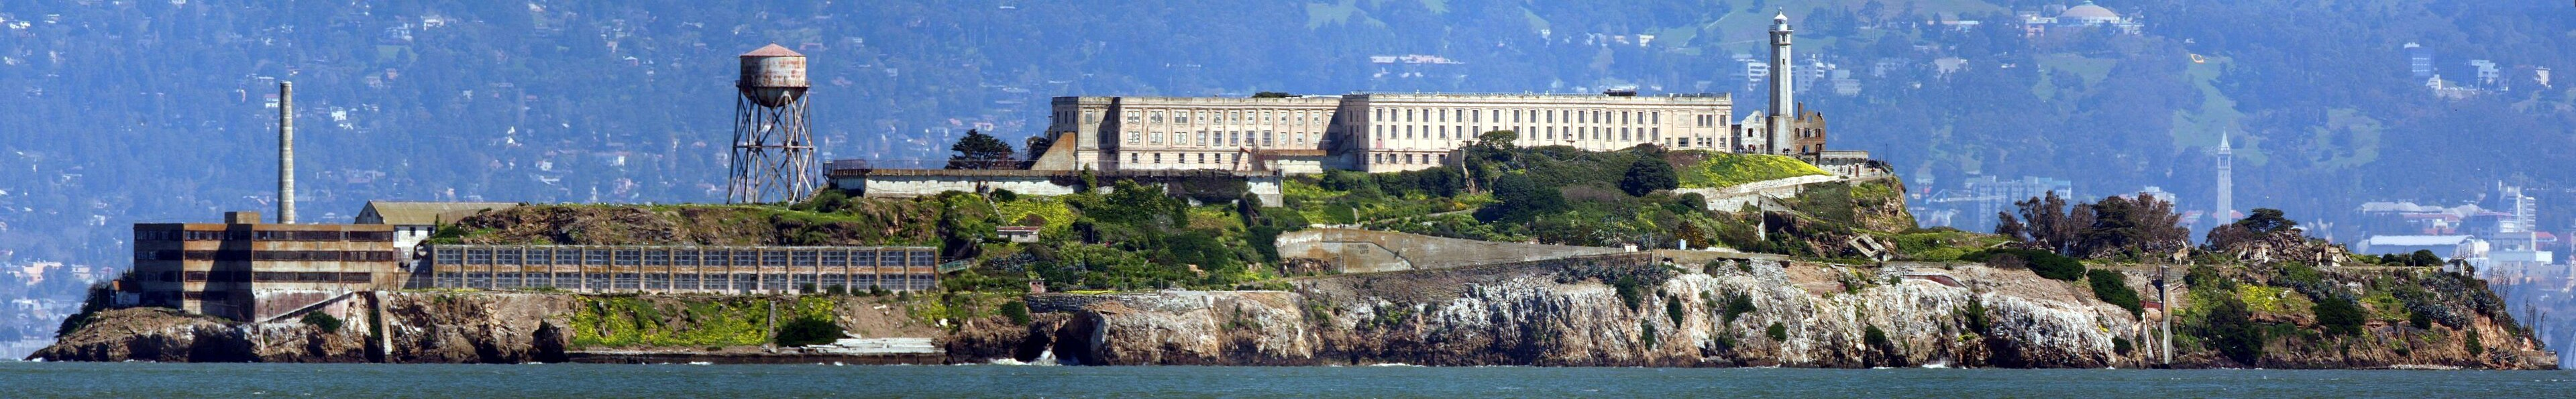
\includegraphics[width=1\linewidth]{images/part4/Alcatraz.png}
    \caption{Alcatraz Island, shown in a panorama created by image stitching}
\end{figure}

\textbf{Overview.} Panorama creation stitches overlapping photographs captured from (approximately) the same optical centre into a single wide-angle composite. Standard pipeline: \textbf{(1)} detect and match features across image pairs; \textbf{(2)} robustly estimate a homography per pair via RANSAC+DLT; \textbf{(3)} project all images onto a common surface (plane, cylinder, or sphere); \textbf{(4)} warp and composite; \textbf{(5)} blend seams. A homography relates two images whenever the camera undergoes a \emph{pure rotation} (fixed optical centre) or the scene is \emph{planar}.\\

\textbf{Homography Estimation - Direct Linear Transform (DLT).} Given $n \ge 4$ point correspondences $\{\mathbf{x}_i \leftrightarrow \mathbf{x}_i'\}$, DLT finds $H$ by forming a homogeneous linear system. Since $\tilde{\mathbf{x}}_i' \sim H\tilde{\mathbf{x}}_i$ (homogeneous equality), the cross-product condition
$$\tilde{\mathbf{x}}_i' \times H\tilde{\mathbf{x}}_i = \mathbf{0}$$
expands (for $\tilde{\mathbf{x}}_i=(x_i,y_i,1)^T$ and $\tilde{\mathbf{x}}_i'=(x_i',y_i',1)^T$) to two independent equations:
$$A_i\,\mathbf{h} = \mathbf{0}, \qquad A_i = \begin{bmatrix} \mathbf{0}^T & -\tilde{\mathbf{x}}_i^T & y_i'\,\tilde{\mathbf{x}}_i^T \\ \tilde{\mathbf{x}}_i^T & \mathbf{0}^T & -x_i'\,\tilde{\mathbf{x}}_i^T \end{bmatrix} \in \mathbb{R}^{2\times9},$$
where $\mathbf{h} = (h_{11},h_{12},\ldots,h_{33})^T \in \mathbb{R}^9$. Stacking all $n$ correspondences:
$$A\mathbf{h} = \mathbf{0}, \quad A\in\mathbb{R}^{2n\times9}.$$
The solution is the \emph{right singular vector} of $A$ for the \emph{smallest singular value} (via SVD), minimizing $\|A\mathbf{h}\|$ subject to $\|\mathbf{h}\|=1$. With $n=4$ correspondences $A$ is $8\times9$, the null space is one-dimensional, and $H$ is determined up to scale (8 DOF).

\begin{figure}[H]
    \centering
    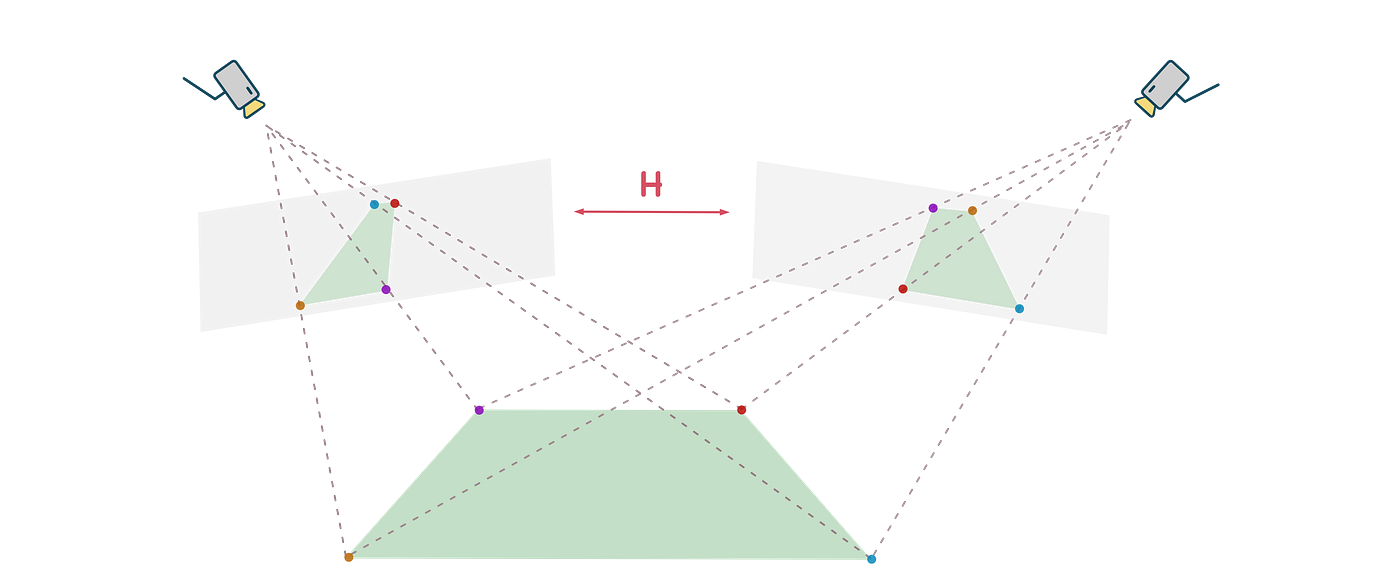
\includegraphics[width=0.75\linewidth]{images/part4/homography-estimation.png}
    \caption{Homography Estimation}
\end{figure}


\textbf{Normalization (essential).} Raw pixel coordinates (spanning hundreds to thousands of units) make $A$ severely ill-conditioned. Before forming $A$, independently normalize each point set:
\begin{enumerate}
    \item Translate so the centroid is at the origin: 
    $$\bar{\mathbf{x}}_i = \mathbf{x}_i - \boldsymbol{\mu}$$
    \item Scale uniformly so the mean distance from the origin is $\sqrt{2}$: 
    $$s = \sqrt{2}/\overline{\|\bar{\mathbf{x}}_i\|}$$
    \item The normalisation matrix is 
    $$T = \begin{bmatrix} s & 0 & -s\mu_x \\ 0 & s & -s\mu_y \\ 0 & 0 & 1 \end{bmatrix}$$
\end{enumerate}
Run DLT on $\hat{\mathbf{x}}_i = T\mathbf{x}_i$ and $\hat{\mathbf{x}}_i' = T'\mathbf{x}_i'$ to obtain $\hat{H}$; then denormalise: $H = T'^{-1}\hat{H}T$. Normalisation reduces condition numbers by orders of magnitude and is mandatory for numerical reliability (Hartley, 1997).\\

\textbf{RANSAC for robust estimation.} Descriptor matching yields many outliers. RANSAC applies with minimum sample $s=4$ (to fit $H$) and inlier threshold $\epsilon \approx 3$ pixels on reprojection error $\|\mathbf{x}_i' - H\mathbf{x}_i\|$. After RANSAC, refit $H$ on all inliers via DLT. Required iterations: $k = \log(1-p)/\log(1-(1-e)^4)$; for $e=0.5$, $p=0.99$: $k\approx72$.\\

\textbf{Non-linear refinement.} DLT minimises an \emph{algebraic} error with no geometric meaning. For higher accuracy, refine $H$ by minimising the \textbf{symmetric reprojection error}:
$$\min_H \sum_i \Bigl(d\!\left(\mathbf{x}_i',\,H\mathbf{x}_i\right)^2 + d\!\left(\mathbf{x}_i,\,H^{-1}\mathbf{x}_i'\right)^2\Bigr),$$
solved by Levenberg--Marquardt initialised from the DLT solution.\\

\textbf{Cylindrical projection.} For wide-angle panoramas ($>\!60°$ field of view), projective stitching produces severe distortion near the periphery. Instead, project each image onto a \emph{cylinder} of radius $f$ (focal length in pixels). For a point $(x,y)$ with origin at the image center:
$$\hat{x} = f\arctan\!\left(\tfrac{x}{f}\right), \qquad \hat{y} = \frac{fy}{\sqrt{x^2+f^2}}.$$
In cylindrical coordinates, a pure camera rotation about the vertical axis becomes a \emph{horizontal translation}, making alignment trivial for rotation-only sequences. The focal length $f$ must be known (from calibration or EXIF).\\

\textbf{Spherical projection.} For full $360°\times180°$ panoramas, project onto a sphere of radius $f$. Spherical angles of image point $(x,y)$:
$$\phi = \arctan\!\left(\tfrac{x}{f}\right), \qquad \lambda = \arctan\!\left(\tfrac{y}{\sqrt{x^2+f^2}}\right).$$
Re-project to \emph{equirectangular} (longitude--latitude) format: $(\phi,\lambda)\to(f\phi,\,f\lambda)$. Used in 360° video, VR headsets, and Google Street View.\\

\textbf{Image blending.} Warped images must be composited; seams appear due to exposure differences, vignetting, and sub-pixel misalignment.

\textit{Alpha feathering.} Assign each pixel a weight $w(\mathbf{x})$ proportional to its distance from the image boundary. In overlap regions blend linearly:
$$C(\mathbf{x}) = \frac{w_A(\mathbf{x})\,C_A(\mathbf{x}) + w_B(\mathbf{x})\,C_B(\mathbf{x})}{w_A(\mathbf{x}) + w_B(\mathbf{x})}.$$
Simple to implement; can produce ghosting under misalignment.

\textit{Multiband blending (Burt \& Adelson, 1983).} Low-frequency content should be blended with a wide transition (to hide color shifts); high-frequency content should be cut sharply (to preserve edge sharpness). Algorithm:
\begin{enumerate}
    \item Build Gaussian pyramids $G_A^{(\ell)}$, $G_B^{(\ell)}$ and mask pyramid $G_M^{(\ell)}$.
    \item Build Laplacian pyramids: $L_A^{(\ell)} = G_A^{(\ell)} - \mathrm{up}(G_A^{(\ell+1)})$, similarly $L_B^{(\ell)}$.
    \item Blend each level: $L_S^{(\ell)} = G_M^{(\ell)}\cdot L_A^{(\ell)} + (1-G_M^{(\ell)})\cdot L_B^{(\ell)}$.
    \item Collapse the blended Laplacian pyramid to reconstruct the composite.
\end{enumerate}

\textit{Seam finding (graph cut).} Rather than blending the entire overlap, find a \emph{minimum-cost cut} through the overlap where the two images agree most closely (minimum photometric difference). Kwatra et al.\ (2003) formulate this as a Markov Random Field and solve with graph cuts, eliminating ghosting entirely.\\

\textbf{Bundle adjustment for multi-image panoramas.} With $m>2$ images, composing pairwise homographies accumulates drift. Global alignment parameterises each camera by its rotation $R_i\in SO(3)$ and focal length $f_i$, then jointly minimises total reprojection error over all matched image pairs $(i,j)$ and inlier correspondences $k$:
$$\min_{\{R_i,\,f_i\}} \sum_{(i,j)\in\mathcal{E}}\;\sum_{k\in\mathcal{M}_{ij}} \left\|\mathbf{x}_k^{(j)} - \pi\!\left(R_j R_i^{-1}\,\pi^{-1}\!\left(\mathbf{x}_k^{(i)};\,f_i\right);\,f_j\right)\right\|^2,$$
where $\pi(\cdot;\,f)$ is projection with focal length $f$ and $\pi^{-1}$ back-projects to 3D. Solved by Levenberg--Marquardt (AutoStitch, Brown \& Lowe, 2007). \textbf{Gain compensation} (per-image exposure scale $g_i$) is typically added to the objective to handle photometric inconsistency between images.







\columnbreaknofill

\NoteChapter{The Pinhole Camera Model}

A camera is a device that maps the 3-D world onto a 2-D image sensor.
The \textbf{pinhole camera} is the simplest mathematical model of this process:
all light rays pass through a single point (the \emph{pinhole}) before hitting
the image plane.  Despite its simplicity, this model underlies virtually all modern computer vision geometry.\\

The complete mapping from a 3-D world point $\mathbf{X}_w$ to a 2-D image
point $\mathbf{x}$ is written compactly as
\[
  \mathbf{x} \sim P\,\mathbf{X}_w,
\]
where $P$ is a $3\times 4$ \textbf{camera matrix} and ``$\sim$'' denotes
equality up to a non-zero scale (homogeneous equality).

\NoteSection{Physical Setup and Coordinate Systems}

\NoteSubsection{Physical components}

\begin{itemize}[noitemsep]
  \item \textbf{Aperture (pinhole):} the single point through which all light
        rays must pass.  Making it infinitely small gives a perfectly sharp
        image but admits no light; real cameras use a finite aperture and a
        lens to focus.
  \item \textbf{Image plane:} the sensor surface at distance $f$ behind the
        pinhole where the image forms.  Each scene point traces a straight ray
        through the pinhole and lands on the image plane.
  \item \textbf{Camera center (optical center / center of projection):} the
        pinhole location itself; the geometric origin of the model.  All
        projection rays emanate from here.
  \item \textbf{Focal length $f$:} the distance from the pinhole to the image
        plane.  A larger $f$ magnifies the image (telephoto); a smaller $f$
        widens the field of view (wide-angle).
  \item \textbf{Principal axis (optical axis):} the ray through the camera
        center perpendicular to the image plane.
  \item \textbf{Principal point $(p_x, p_y)$:} where the principal axis
        intersects the image plane.  Ideally the image center, but shifts due
        to manufacturing imperfections.
\end{itemize}

\NoteSubsection{Three coordinate frames}

Three reference frames are needed to describe the full projection pipeline:

\begin{itemize}[noitemsep]
  \item \textbf{World frame} $(\widetilde{\mathbf{X}}_w)$: a fixed global
        frame in which 3-D scene points are defined.  Arbitrary choice.
  \item \textbf{Camera frame} $(\widetilde{\mathbf{X}}_c)$: origin at the
        camera center, $z$-axis along the principal axis pointing into the
        scene.  The natural frame for projection.
  \item \textbf{Image frame} $(u, v)$: 2-D pixel coordinates on the sensor,
        with origin at the image corner (not the principal point).
\end{itemize}

The full pipeline is:
\[
  \underbrace{\widetilde{\mathbf{X}}_w}_{\text{world}}
  \;\xrightarrow[\text{extrinsics}]{[\mathbf{R}\mid\mathbf{t}]}\;
  \underbrace{\widetilde{\mathbf{X}}_c}_{\text{camera}}
  \;\xrightarrow[\text{projection}]{\text{divide by }z}\;
  \underbrace{(x_n, y_n)}_{\text{normalized}}
  \;\xrightarrow[\text{intrinsics}]{K}\;
  \underbrace{(u, v)}_{\text{pixel}}.
\]

\begin{figure}[H]
    \centering
    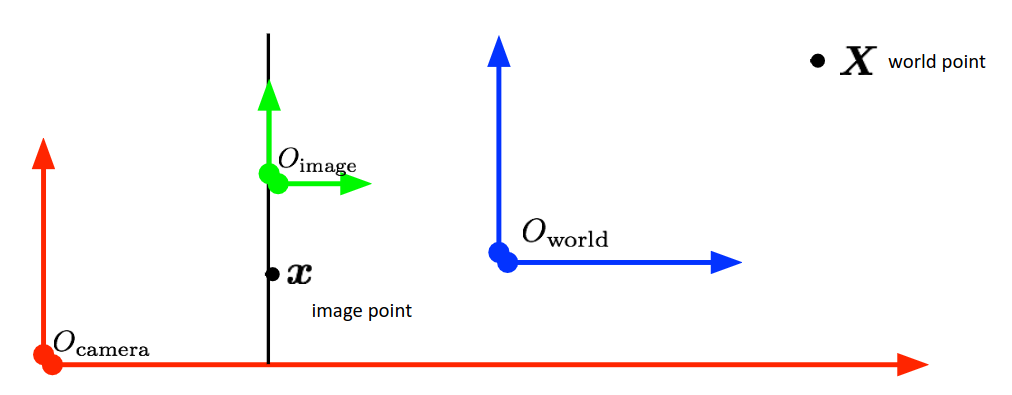
\includegraphics[width=0.75\linewidth]{images/part4/world-to-camera.png}
\end{figure}

\NoteSection{Perspective Projection}

\NoteSubsection{Derivation from similar triangles}

Place the camera center at the origin with the image plane at $z = f$.
A 3-D point in camera coordinates $\widetilde{\mathbf{X}}_c = (X, Y, Z)^\top$
emits a ray through the origin.  That ray intersects the image plane at the
2-D point $(x, y)$.

By similar triangles along both axes:
\[
  \frac{x}{f} = \frac{X}{Z}
  \;\Longrightarrow\; x = \frac{fX}{Z},
  \qquad
  \frac{y}{f} = \frac{Y}{Z}
  \;\Longrightarrow\; y = \frac{fY}{Z}.
\]

This is the \textbf{perspective projection} (also called \emph{central
projection}):
\begin{equation}
  \begin{pmatrix} X \\ Y \\ Z \end{pmatrix}
  \;\longmapsto\;
  \begin{pmatrix} fX/Z \\ fY/Z \end{pmatrix}.
  \label{eq:persp-proj}
\end{equation}

Two key consequences follow immediately:
\begin{itemize}[noitemsep]
  \item \textbf{Depth-dependent scaling:} farther objects appear smaller
        (magnification $m = f/Z$ decreases with $Z$).
  \item \textbf{Nonlinearity:} the division by $Z$ makes perspective projection
        nonlinear in Euclidean coordinates.  Homogeneous coordinates linearize it.
\end{itemize}

\NoteSubsection{Normalized image coordinates ($f=1$)}

Setting $f = 1$ and placing the image plane at $z = 1$ gives the
\emph{normalized} (or \emph{canonical}) projection:
\begin{equation}
  (X, Y, Z)^\top \;\longmapsto\; (X/Z,\; Y/Z)^\top.
  \label{eq:norm-proj}
\end{equation}
These \textbf{normalized image coordinates} $(x_n, y_n) = (X/Z, Y/Z)$ are
independent of any camera-specific parameters and form the intermediate
representation before applying the intrinsic matrix $K$.

\NoteSection{Camera Matrix and Homogeneous Coordinates}

\NoteSubsection{Why homogeneous coordinates?}

Perspective projection involves division by $Z$, which is nonlinear.
\textbf{Homogeneous coordinates} represent a 2-D point $(u,v)$ as a
3-vector $(u, v, 1)^\top$ (or any non-zero scalar multiple thereof), and
a 3-D point $(X,Y,Z)$ as a 4-vector $(X, Y, Z, 1)^\top$.  This trick
turns perspective projection into a \emph{linear} matrix multiplication:
the division by $Z$ is deferred and recovered by dividing out the last
coordinate at the end (``de-homogenization'').

\NoteSubsection{Camera as a linear map}

A camera maps homogeneous 3-D world coordinates to homogeneous 2-D image
coordinates:
\begin{equation}
  \mathbf{x} \sim \mathbf{P}\,\mathbf{X}_w,
  \qquad
  \mathbf{x} \in \mathbb{P}^2,\quad \mathbf{X}_w \in \mathbb{P}^3,
\end{equation}
where $\mathbf{P}$ is the $3\times 4$ \textbf{camera matrix} (11 DOF after
removing the overall scale ambiguity from 12 entries).  Expanded:
\[
\begin{pmatrix}
    \tilde{u} \\ \tilde{v} \\ \tilde{w}
\end{pmatrix}
=
\begin{pmatrix}
    p_{11} & p_{12} & p_{13} & p_{14} \\
    p_{21} & p_{22} & p_{23} & p_{24} \\
    p_{31} & p_{32} & p_{33} & p_{34}
\end{pmatrix}
\begin{pmatrix}
    X \\ Y \\ Z \\ 1
\end{pmatrix},
\qquad
(u,v) = \left(\frac{\tilde{u}}{\tilde{w}},\, \frac{\tilde{v}}{\tilde{w}}\right).
\]

\NoteSubsection{Simplest projection matrix ($f=1$, camera at origin)}

When the camera center coincides with the world origin and $f = 1$:
\begin{equation}
  P_0 = \bigl[\,I_{3\times 3} \mid \mathbf{0}\,\bigr]
      = \begin{pmatrix}
          1 & 0 & 0 & 0 \\
          0 & 1 & 0 & 0 \\
          0 & 0 & 1 & 0
        \end{pmatrix}.
\end{equation}
Applying $P_0$ to $(X, Y, Z, 1)^\top$ yields $(X, Y, Z)^\top$ in homogeneous
image coordinates, which de-homogenizes to $(X/Z, Y/Z)^\top$, recovering
the normalized projection~\eqref{eq:norm-proj}.

\NoteSubsection{General focal length $f$}

Scaling the first two rows by $f$ encodes the image-plane distance:
\begin{equation}
  P_f = \begin{pmatrix}
    f & 0 & 0 & 0 \\
    0 & f & 0 & 0 \\
    0 & 0 & 1 & 0
  \end{pmatrix},
  \qquad
  (X,Y,Z,1)^\top \mapsto (fX/Z,\; fY/Z)^\top,
\end{equation}
recovering the full perspective equation~\eqref{eq:persp-proj}.

\NoteSection{Intrinsic Matrix $K$}

The \textbf{intrinsic matrix} $K$ converts normalized image coordinates
$(x_n, y_n)$ to pixel coordinates $(u, v)$.  It bundles all
camera-internal geometric parameters.

\NoteSubsection{Principal-point offset}

The image origin is typically at the sensor corner, not at the principal
point.  Adding offset $(p_x, p_y)$ in pixels:
\begin{equation}
  u = f\,x_n + p_x, \qquad v = f\,y_n + p_y.
\end{equation}
This gives the standard $K$ for a camera with square pixels:
\begin{equation}
  K = \begin{pmatrix}
    f   & 0 & p_x \\
    0   & f & p_y \\
    0   & 0 & 1
  \end{pmatrix}.
\end{equation}
Intrinsic DOF: $f$ (1) $+$ $p_x, p_y$ (2) $=$ 3 intrinsic parameters.
With 6 extrinsic DOF ($\mathbf{R}$: 3, $\mathbf{t}$: 3), the standard
model has $\mathbf{9}$ DOF total.

\NoteSubsection{CCD camera --- non-square pixels}

Digital sensors may have non-square pixels, giving separate effective focal
lengths $f_x$ and $f_y$ (in pixels) along each axis:
\begin{equation}
  K = \begin{pmatrix}
    f_x & 0   & p_x \\
    0   & f_y & p_y \\
    0   & 0   & 1
  \end{pmatrix}, \qquad f_x = f\,s_x,\quad f_y = f\,s_y,
\end{equation}
where $s_x, s_y$ are the pixel densities (pixels per meter).  Adding
$f_y$ as a free parameter brings the intrinsic count to 4, giving
\textbf{10 DOF} total.

\NoteSubsection{Finite projective camera --- sensor skew}

If the pixel axes are not exactly perpendicular (e.g., due to
manufacturing imperfections), a \textbf{skew} parameter $s$ couples the
$x$ and $y$ directions:
\begin{equation}
  K = \begin{pmatrix}
    f_x & s   & p_x \\
    0   & f_y & p_y \\
    0   & 0   & 1
  \end{pmatrix}, \qquad s \neq 0.
\end{equation}
In practice $s \approx 0$ for modern sensors, but the general model with
all 5 intrinsic parameters free gives \textbf{11 DOF} total.  This is the
most general \emph{finite} camera (infinite cameras such as orthographic
are excluded).

\NoteSubsection{Degrees-of-freedom summary}

\begin{center}
\begin{tabular}{lccc}
  \toprule
  Camera model & Intrinsic params & Extra & Total DOF \\
  \midrule
  Standard pinhole        & $f, p_x, p_y$         & ---       & 9  \\
  CCD (non-square pixels) & $f_x, f_y, p_x, p_y$  & $f_y$     & 10 \\
  Finite projective (skew)& $f_x, f_y, s, p_x, p_y$ & $s$    & 11 \\
  \bottomrule
\end{tabular}
\end{center}

\noindent Extrinsic DOF (6) = rotation (3) + translation (3) in all cases.

\NoteSection{Extrinsic Parameters}

\NoteSubsection{World-to-camera coordinate transform}

The \textbf{extrinsic parameters} describe the camera's pose (position and
orientation) in the world.  They transform world coordinates into camera
coordinates before projection.

Let $\widetilde{\mathbf{C}} \in \mathbb{R}^3$ be the camera center's
position in world coordinates, and $\mathbf{R} \in SO(3)$ be the
$3\times 3$ rotation matrix whose columns are the world-frame directions
of the camera's $x$-, $y$-, and $z$-axes.

The world-to-camera transform in Euclidean coordinates is:
\begin{equation}
  \widetilde{\mathbf{X}}_c
  = \mathbf{R}\!\left(\widetilde{\mathbf{X}}_w - \widetilde{\mathbf{C}}\right)
  = \mathbf{R}\,\widetilde{\mathbf{X}}_w \underbrace{- \mathbf{R}\widetilde{\mathbf{C}}}_{\mathbf{t}}.
\end{equation}

\textit{Key insight:} $\mathbf{t} = -\mathbf{R}\widetilde{\mathbf{C}}$
is \emph{not} the camera position but rather the position of the world
origin in camera coordinates.

In homogeneous block form ($4\times 4$), this is an invertible rigid-body
transform:
\begin{equation}
  \mathbf{X}_c
  = \underbrace{\begin{pmatrix} \mathbf{R} & -\mathbf{R}\widetilde{\mathbf{C}} \\
                  \mathbf{0}^\top & 1 \end{pmatrix}}_{[\mathbf{R}\mid\mathbf{t}]_{\text{homog.}}}
    \mathbf{X}_w.
\end{equation}

\NoteSubsection{Recovering the camera center from $\mathbf{t}$}

Given the compact parameterization $P = K[\mathbf{R}\mid\mathbf{t}]$,
the camera center in world coordinates is recovered as:
\begin{equation}
  \widetilde{\mathbf{C}} = -\mathbf{R}^\top\,\mathbf{t}.
\end{equation}

\NoteSection{Full Camera Matrix}

\NoteSubsection{Assembling the pipeline}

The complete projection from world point to pixel is:
\begin{align}
  \mathbf{X}_c &= \bigl[\mathbf{R}\mid\mathbf{t}\bigr]\,\mathbf{X}_w
    & &\text{(extrinsics: world $\to$ camera)} \\
  \mathbf{x}_n &= P_0\,\mathbf{X}_c
    & &\text{(ideal projection with }f=1\text{)} \\
  \mathbf{x}   &= K\,\mathbf{x}_n
    & &\text{(intrinsics: normalized $\to$ pixel).}
\end{align}
Chaining these three steps gives the canonical decomposition of $P$:
\begin{equation}
  \boxed{
    P = K\,\bigl[I \mid \mathbf{0}\bigr]
        \begin{pmatrix} \mathbf{R} & -\mathbf{R}\widetilde{\mathbf{C}} \\
                        \mathbf{0}^\top & 1 \end{pmatrix}
      = K\,[\,\mathbf{R} \mid \mathbf{t}\,],
    \qquad \mathbf{t} = -\mathbf{R}\widetilde{\mathbf{C}}.
  }
\end{equation}

The left $3\times 3$ block of $P$ is $M = K\mathbf{R}$, the product of
an upper-triangular matrix ($K$) and an orthogonal matrix ($\mathbf{R}$).
This structure enables later decomposition via QR.

\NoteSubsection{Block-size summary}

\begin{center}
\begin{tabular}{@{}llll@{}}
  \toprule
  Block & Size & Structure & Physical meaning \\
  \midrule
  $K$           & $3\times 3$ & upper-triangular    & intrinsic camera geometry \\
  $\mathbf{R}$  & $3\times 3$ & orthogonal $SO(3)$  & camera orientation in world \\
  $\mathbf{t}$  & $3\times 1$ & vector              & world origin in camera frame \\
  $P$           & $3\times 4$ & general rank-3      & full projection matrix \\
  \bottomrule
\end{tabular}
\end{center}

\NoteSection{Perspective Distortion}

\NoteSubsection{Depth-dependent magnification}

The image magnification at depth $Z$ is:
\begin{equation}
  m(Z) = \frac{f}{Z}.
\end{equation}
Because $m$ depends on $Z$, objects at different depths are scaled
differently.  This is \textbf{perspective distortion}: parallel lines
converge to \emph{vanishing points}, and depth changes cause apparent
size changes even for rigid objects.

\NoteSubsection{The dolly-zoom (Vertigo) effect}

Doubling $f$ while simultaneously doubling $Z$ keeps the foreground
subject at the same image size ($m = f/Z = \text{const}$), but
background objects --- at a different depth $Z'$ --- are now magnified by
$f'/(Z') = 2f/Z'$, making them appear compressed relative to the
foreground.  This is the basis of the \textbf{dolly-zoom} (``Vertigo
effect'') in cinematography.

\NoteSubsection{Foreshortening and vanishing points}

A set of parallel lines in the world with direction vector $\mathbf{d}$
converges in the image to a single \textbf{vanishing point} at
$\mathbf{v} = K\mathbf{R}\mathbf{d}$ (in homogeneous coordinates).
The horizon line is the set of all vanishing points for horizontal
directions, lying at the image row corresponding to the camera's eye level.

\NoteSection{Alternative Camera Models}

\NoteSubsection{Weak perspective (scaled orthographic)}

When the scene depth variation $\Delta Z$ is small compared to the
average depth $Z_0$ (i.e., $\Delta Z \ll Z_0$), all points are
approximated as being at the same depth $Z_0$.  The depth-dependent
magnification $f/Z$ is then replaced by a single constant scale factor
$m = f/Z_0$:
\begin{equation}
  (X, Y, Z)^\top \;\longmapsto\; (mX,\; mY)^\top,
  \qquad m = \frac{f}{Z_0},
\end{equation}
\begin{equation}
  P_{\text{weak}} =
  \begin{pmatrix}
    m & 0 & 0 & 0 \\
    0 & m & 0 & 0 \\
    0 & 0 & 0 & 1
  \end{pmatrix}.
\end{equation}
This is valid when (1) the scene is very far from the camera, or (2) a
\textbf{telecentric lens} is used (pinhole placed at the front focal
point, admitting only rays parallel to the principal axis).

\NoteSubsection{Orthographic projection}

The special case of weak perspective with $m = 1$ and no origin offset
gives pure \textbf{orthographic projection}: depth is entirely ignored,
and world $x, y$ coordinates map directly to image coordinates.
\begin{equation}
  P_{\text{ortho}} =
  \begin{pmatrix}
    1 & 0 & 0 & 0 \\
    0 & 1 & 0 & 0 \\
    0 & 0 & 0 & 1
  \end{pmatrix}.
\end{equation}
Orthographic projection preserves parallel lines, distances, and ratios
along any direction --- properties lost in perspective projection.
It is accurate for engineering/CAD drawings and telephoto photography of
distant objects.

\NoteSection{Pose Estimation and Camera Calibration}

\textbf{Goal:} Given $N$ point correspondences
$\bigl\{(\mathbf{X}_i,\,\mathbf{x}_i)\bigr\}_{i=1}^{N}$ between known
3-D world points and observed 2-D image points, estimate the $3\times 4$
camera matrix $P$.

\NoteSubsection{Projection equations in inhomogeneous coordinates}

Let $\mathbf{m}_j^\top$ denote the $j$-th row of $P$ (a $1\times 4$
vector).  The projection $\mathbf{x}_i = P\,\mathbf{X}_i$ in homogeneous
form de-homogenizes to:
\begin{equation}
  u_i = \frac{\mathbf{m}_1^\top\,\mathbf{X}_i}{\mathbf{m}_3^\top\,\mathbf{X}_i},
  \qquad
  v_i = \frac{\mathbf{m}_2^\top\,\mathbf{X}_i}{\mathbf{m}_3^\top\,\mathbf{X}_i}.
  \label{eq:proj-het}
\end{equation}
These are rational (nonlinear) functions of $P$'s entries due to the
shared denominator $\mathbf{m}_3^\top\mathbf{X}_i$.

\NoteSubsection{Linearization: Direct Linear Transform (DLT)}

Cross-multiplying~\eqref{eq:proj-het} clears the denominator and yields
two \emph{linear} equations per correspondence:
\begin{align}
  \mathbf{m}_1^\top\,\mathbf{X}_i - u_i\,\mathbf{m}_3^\top\,\mathbf{X}_i &= 0, \\
  \mathbf{m}_2^\top\,\mathbf{X}_i - v_i\,\mathbf{m}_3^\top\,\mathbf{X}_i &= 0.
\end{align}
Stacking these for all $N$ correspondences into a matrix $A \in \mathbb{R}^{2N\times 12}$:
\begin{equation}
  A\,\mathbf{p} = \mathbf{0}, \qquad \mathbf{p} = \operatorname{vec}(P) \in \mathbb{R}^{12}.
\end{equation}
This is a homogeneous linear system: the camera matrix $P$ lies in the
null space of $A$.  Since $P$ has 11 DOF (12 entries, 1 scale), each
correspondence contributes 2 constraints, so $N \geq 6$ correspondences
are needed (actually $N=6$ gives exactly 11 constraints; more gives an
overdetermined system solved in the least-squares sense).

\NoteSubsection{Solution by SVD}

The minimum-norm solution (constrained to $\|\mathbf{p}\|=1$ to avoid
the trivial $\mathbf{p}=\mathbf{0}$) is:
\begin{equation}
  \hat{\mathbf{p}} = \arg\min_{\|\mathbf{p}\|=1} \|A\mathbf{p}\|^2
  = \text{last column of } V \text{ in } A = U\Sigma V^\top.
\end{equation}
Equivalently, $\hat{\mathbf{p}}$ is the eigenvector of $A^\top A$
corresponding to its \emph{smallest} eigenvalue.  This is the
\textbf{DLT algorithm}.

\NoteSection{Camera Matrix Decomposition}

Given an estimated $P$, it is useful to recover the physical parameters
$K$, $\mathbf{R}$, and $\widetilde{\mathbf{C}}$ separately.

\NoteSubsection{Recovering the camera center $\widetilde{\mathbf{C}}$}

By definition, the camera center projects to the zero vector under $P$:
\begin{equation}
  P\,\widetilde{\mathbf{C}}_h = \mathbf{0}
  \;\Longrightarrow\;
  \widetilde{\mathbf{C}}_h = \operatorname{null}(P).
\end{equation}
Numerically, $\widetilde{\mathbf{C}}_h$ is the right singular vector of
$P$ corresponding to the smallest singular value (from $P = U\Sigma V^\top$,
take the last column of $V$).  De-homogenize to get $\widetilde{\mathbf{C}}$.

\NoteSubsection{Recovering intrinsics $K$ and rotation $\mathbf{R}$}

Write $P = [M \mid \mathbf{p}_4]$ where $M = K\mathbf{R}$ is the
left $3\times 3$ block.  Since $K$ is upper-triangular with positive
diagonal and $\mathbf{R}$ is orthogonal, their product $M$ has a unique
factorization via \textbf{RQ decomposition} (a variant of QR):
\begin{equation}
  M = K\mathbf{R}
  \;\xrightarrow{\;\text{RQ}\;}
  K \;\text{(upper-triangular, positive diagonal)},\quad
  \mathbf{R} \;\text{(orthogonal)}.
\end{equation}
Finally, $\mathbf{t} = K^{-1}\mathbf{p}_4$, and the camera center is
$\widetilde{\mathbf{C}} = -\mathbf{R}^\top\mathbf{t}$.

\NoteSection{Nonlinear Refinement and Lens Distortion}

\NoteSubsection{Reprojection error}

The DLT solution minimizes an algebraic error that has no direct geometric
meaning.  The preferred objective is the \textbf{reprojection error} ---
the sum of squared Euclidean distances between observed image points and
their projections under the estimated $P$:
\begin{equation}
  E(K,\mathbf{R},\mathbf{t}) = \sum_{i=1}^{N}
      \left[
        \left(u_i - \frac{\mathbf{m}_1^\top\,\mathbf{X}_i}
                         {\mathbf{m}_3^\top\,\mathbf{X}_i}\right)^{\!2}
        +
        \left(v_i - \frac{\mathbf{m}_2^\top\,\mathbf{X}_i}
                         {\mathbf{m}_3^\top\,\mathbf{X}_i}\right)^{\!2}
      \right].
\end{equation}
Minimized over $K$, $\mathbf{R}$, $\mathbf{t}$ by iterative nonlinear
optimization (typically Levenberg--Marquardt), initialized from the DLT
solution.

\NoteSubsection{Radial lens distortion}

Real lenses deviate from the ideal pinhole model.  The dominant
imperfection is \textbf{radial distortion}: image points are displaced
radially from the principal point.  Let $(x_n, y_n)$ be ideal normalized
coordinates and $r^2 = x_n^2 + y_n^2$.  The distorted normalized coordinates are:

\begin{align}
    x_d &= x_n\,(1 + k_1 r^2 + k_2 r^4 + k_3 r^6 + \cdots),\\
    y_d &= y_n\,(1 + k_1 r^2 + k_2 r^4 + k_3 r^6 + \cdots),
\end{align}

where $k_1, k_2, k_3$ are \textbf{radial distortion coefficients}
estimated during calibration.

\begin{itemize}[noitemsep]
  \item \textbf{Barrel distortion ($k_1 < 0$):} image bulges outward;
        straight lines bow away from center.  Common in wide-angle lenses.
  \item \textbf{Pincushion distortion ($k_1 > 0$):} image pinches inward;
        straight lines bow toward center.  Common in telephoto lenses.
\end{itemize}

The distorted reprojection error adds distortion correction to the pipeline:
$(x_n, y_n) \to (x_d, y_d) \to K \to (u, v)$.

\NoteSection{Calibration Methods}

\NoteSubsection{Reference-object (3-D target) calibration}

Place an object of precisely known 3-D geometry in the scene (e.g., a
calibration rig with marked corner points), identify corresponding 2-D
image points, and solve via DLT.

\begin{itemize}[noitemsep]
  \item \textbf{Pros:} Closed-form solution; straightforward to implement.
  \item \textbf{Cons:} Requires a precisely manufactured 3-D object;
        does not model radial distortion without extension; cannot impose
        known constraints (e.g., known aspect ratio, zero skew).
\end{itemize}

\NoteSubsection{Multi-plane (Zhang's) calibration}

Photograph a flat planar pattern (e.g., checkerboard) from at least 3
different viewpoints.  Corner positions on the plane are known in 2-D
pattern coordinates; their 3-D positions are inferred from the known
planar structure.  Each viewpoint provides a \textbf{homography} (a
$3\times 3$ projective transform between the plane and the image) from
which constraints on $K$ are extracted.
\begin{itemize}[noitemsep]
  \item \textbf{Pros:} Only requires a printed checkerboard; positions
        and orientations of the board need not be known; handles radial
        distortion; implemented in MATLAB (Bouguet toolbox) and OpenCV.
  \item \textbf{Cons:} Requires at least 3 views; involves nonlinear
        optimization for final refinement.
\end{itemize}

\NoteSection{Augmented Reality Application}

The full camera pipeline is illustrated concretely by a simple AR system:
\begin{enumerate}[noitemsep]
  \item \textbf{Detect} known 2-D feature points on a flat AR marker
        (e.g., a QR-code border or checkerboard).
  \item \textbf{Estimate pose} $[\mathbf{R}\mid\mathbf{t}]$ from the
        2-D$\leftrightarrow$3-D correspondences using DLT followed by
        Levenberg--Marquardt refinement on reprojection error.  $K$ is
        pre-calibrated.
  \item \textbf{Render virtual content} by projecting 3-D virtual geometry
        through the estimated $P = K[\mathbf{R}\mid\mathbf{t}]$:
        \[
          \mathbf{x}_{\text{virtual}} \sim P\,\mathbf{X}_{\text{3D}}.
        \]
  \item \textbf{Composite} the rendered virtual image onto the live camera
        feed, producing the AR output.
\end{enumerate}
The quality of the overlay depends directly on the accuracy of $K$
(calibration) and $[\mathbf{R}\mid\mathbf{t}]$ (pose estimation).





\end{notes}
\end{document}
